%%%%%%%%%%%%%%%%%%%%%%%%%%%%%%%%%%%%%%%%%
% Beamer Presentation
% LaTeX Template
% Version 1.0 (10/11/12)
%
% This template has been downloaded from:
% http://www.LaTeXTemplates.com
%
% License:
% CC BY-NC-SA 3.0 (http://creativecommons.org/licenses/by-nc-sa/3.0/)
%
%%%%%%%%%%%%%%%%%%%%%%%%%%%%%%%%%%%%%%%%%

%----------------------------------------------------------------------------------------
%	PACKAGES AND THEMES
%----------------------------------------------------------------------------------------

\documentclass[t]{beamer}




\mode<presentation> {

% The Beamer class comes with a number of default slide themes
% which change the colors and layouts of slides. Below this is a list
% of all the themes, uncomment each in turn to see what they look like.

%\usetheme{default}
%\usetheme{AnnArbor}
%\usetheme{Antibes}
%\usetheme{Bergen}
%\usetheme{Berkeley}
%\usetheme{Berlin}
%\usetheme{Boadilla}
%\usetheme{CambridgeUS}
%\usetheme{Copenhagen}
%\usetheme{Darmstadt}
%\usetheme{Dresden}
%\usetheme{Frankfurt}
%\usetheme{Goettingen}
%\usetheme{Hannover}
%\usetheme{Ilmenau}
%\usetheme{JuanLesPins}
%\usetheme{Luebeck}
%\usetheme{Madrid}
%\usetheme{Malmoe}
%\usetheme{Marburg}
%\usetheme{Montpellier}
%\usetheme{PaloAlto}
%\usetheme{Pittsburgh}
%\usetheme{Rochester}
%\usetheme{Singapore}
%\usetheme{Szeged}
%\usetheme{Warsaw}

\usetheme{ITS_CI}

% As well as themes, the Beamer class has a number of color themes
% for any slide theme. Uncomment each of these in turn to see how it
% changes the colors of your current slide theme.

%\usecolortheme{albatross}
%\usecolortheme{beaver}
%\usecolortheme{beetle}
%\usecolortheme{crane}
%\usecolortheme{dolphin}
%\usecolortheme{dove}
%\usecolortheme{fly}
%\usecolortheme{lily}
%\usecolortheme{orchid}
%\usecolortheme{rose}
%\usecolortheme{seagull}
%\usecolortheme{seahorse}
%\usecolortheme{whale}
%\usecolortheme{wolverine}

%\setbeamertemplate{footline} % To remove the footer line in all slides uncomment this line
%\setbeamertemplate{footline}[page number] % To replace the footer line in all slides with a simple slide count uncomment this line

\setbeamertemplate{navigation symbols}{} % To remove the navigation symbols from the bottom of all slides uncomment this line
}

\usepackage{amsmath}
\usepackage{textcomp}
\usepackage{anyfontsize}
\usepackage{graphicx} % Allows including images
\usepackage{booktabs} % Allows the use of \toprule, \midrule and \bottomrule in tables
\usepackage{calc}
\usepackage{tikz}
\usepackage{hyphenat}
\usetikzlibrary{arrows,shapes}

\newlength{\okinalen}
\setlength{\okinalen}{\widthof{'}}
\newcommand{\okina}{\hbox to.666\okinalen{\hss`\hss}}

\newcommand{\CNAME}{the~Cray~CS300}
\newcommand{\TOTWRKS}{64}
\newcommand{\ctilde}{{\fontfamily{ptm}\selectfont\texttildelow}}
\newcommand{\itab}[1]{\hspace{0em}\rlap{#1}}
\newcommand{\tab}[1]{\hspace{.2\textwidth}\rlap{#1}}

\definecolor{links}{HTML}{2A1B81}
\hypersetup{colorlinks,linkcolor=,urlcolor=links}



\AtBeginSection[]
               {
                 \begin{frame}
                   \frametitle{Outline}
                   \tableofcontents[currentsection]
                 \end{frame}
               }
               


\AtBeginSubsection[]
                  {
                    \begin{frame}
                      \frametitle{Outline}
                      \tableofcontents[currentsection,currentsubsection]
                    \end{frame}
                  }
                  

%----------------------------------------------------------------------------------------
%	TITLE PAGE
%----------------------------------------------------------------------------------------

\title[MATLAB on \CNAME]{MATLAB Distributed Compute on \CNAME } % The short title appears at the bottom of every slide, the full title is only on the title page

\author{Sean Cleveland Ph.D, Ron Merrill Ph.D,\\David Schanzenbach M.S.} % Your name
\institute[University of Hawai\okina{}i -- ITS--CI] % Your institution as it will appear on the bottom of every slide, may be shorthand to save space
{
	Information Technology Services \\
	Cyberinfrastructure \\
	University of Hawai\okina{}i \\ % Your institution for the title page
	\medskip
	\textbf{\url{https://www.hawaii.edu/its/ci/}}\\
	\textbf{\textit{uh-hpc-help@lists.hawaii.edu}} % Your email address
}
\date{\today} % Date, can be changed to a custom date

          
\begin{document}

\begin{frame}
  \titlepage % Print the title page as the first slide
\end{frame}

\begin{frame}
  \frametitle{Overview} % Table of contents slide, comment this block out to remove it
  \tableofcontents[] % Throughout your presentation, if you choose to use \section{} and \subsection{} commands, these will automatically be printed on this slide as an overview of your presentation
\end{frame}

\section{MATLAB Distributed Compute}

\begin{frame}
	\frametitle{MATLAB on the Cluster}
	\begin{itemize}
		\item MATLAB Distributed Compute Server (DCS) R2015b is installed on \CNAME
		\item We currently hold a license for \TOTWRKS{} \emph{Workers}.
			\begin{itemize}
				\item One worker is equal to an instance of MATLAB
			\end{itemize}
		\item In order to use MATLAB on \CNAME, you will need to own the MATLAB product with the Parallel Computing Toolbox
		\item The workers on \CNAME~contain all the MATLAB toolboxes
		\begin{itemize}
			\item \textbf{This does not mean you get free access to all toolboxes}
			\item \textbf{You will only have access to the MATLAB toolboxes you have purchased}
		\end{itemize}            
	\end{itemize}
\end{frame}


\begin{frame}
  \frametitle{Pre-requisites to using MATLAB on \CNAME{}}
  In order to use MATLAB on the cluster you must meet the follow requirements
  \begin{enumerate}
  \item Own a copy of MATLAB, with a license for the Parallel Computing Toolbox
  \item Have gone through the On-boarding course for \CNAME
  \end{enumerate}
\end{frame}


\section{Configuration}

\begin{frame}
  \frametitle{Required Files}
  In order to submit MATLAB jobs to \CNAME, a packet of several scripts, and a configuration file are required:
  \begin{itemize}
  \item Download the zip file containing the MATLAB setup files here: \url{http://go.hawaii.edu/YH}
  \item Download should contain:
    \begin{itemize}
    \item A directory named slurm\_matlab, which contains several .m and .sh files
    \item A settings file named uhhpc.settings
    \end{itemize}
  \end{itemize}
\end{frame}


\begin{frame}
  \frametitle{Setting up MATLAB}
  \begin{itemize}
  \item Unzip setup files
  \item Move the \emph{slurm\_matlab} directory to a location it can reside permanently
    \begin{itemize}
    \item This directory will be added to your MATLAB path
    \end{itemize}
  \item Start up MATLAB
  \end{itemize}
  The next few Slides will cover what needs to be done in MATLAB to allow communication with \CNAME~from MATLAB
\end{frame}


\subsection{Setting up the MATLAB path}
\begin{frame}
  \frametitle{Adding to the MATLAB Path}
  \begin{picture}(320,250)
    \onslide<1->{\put(-8,92){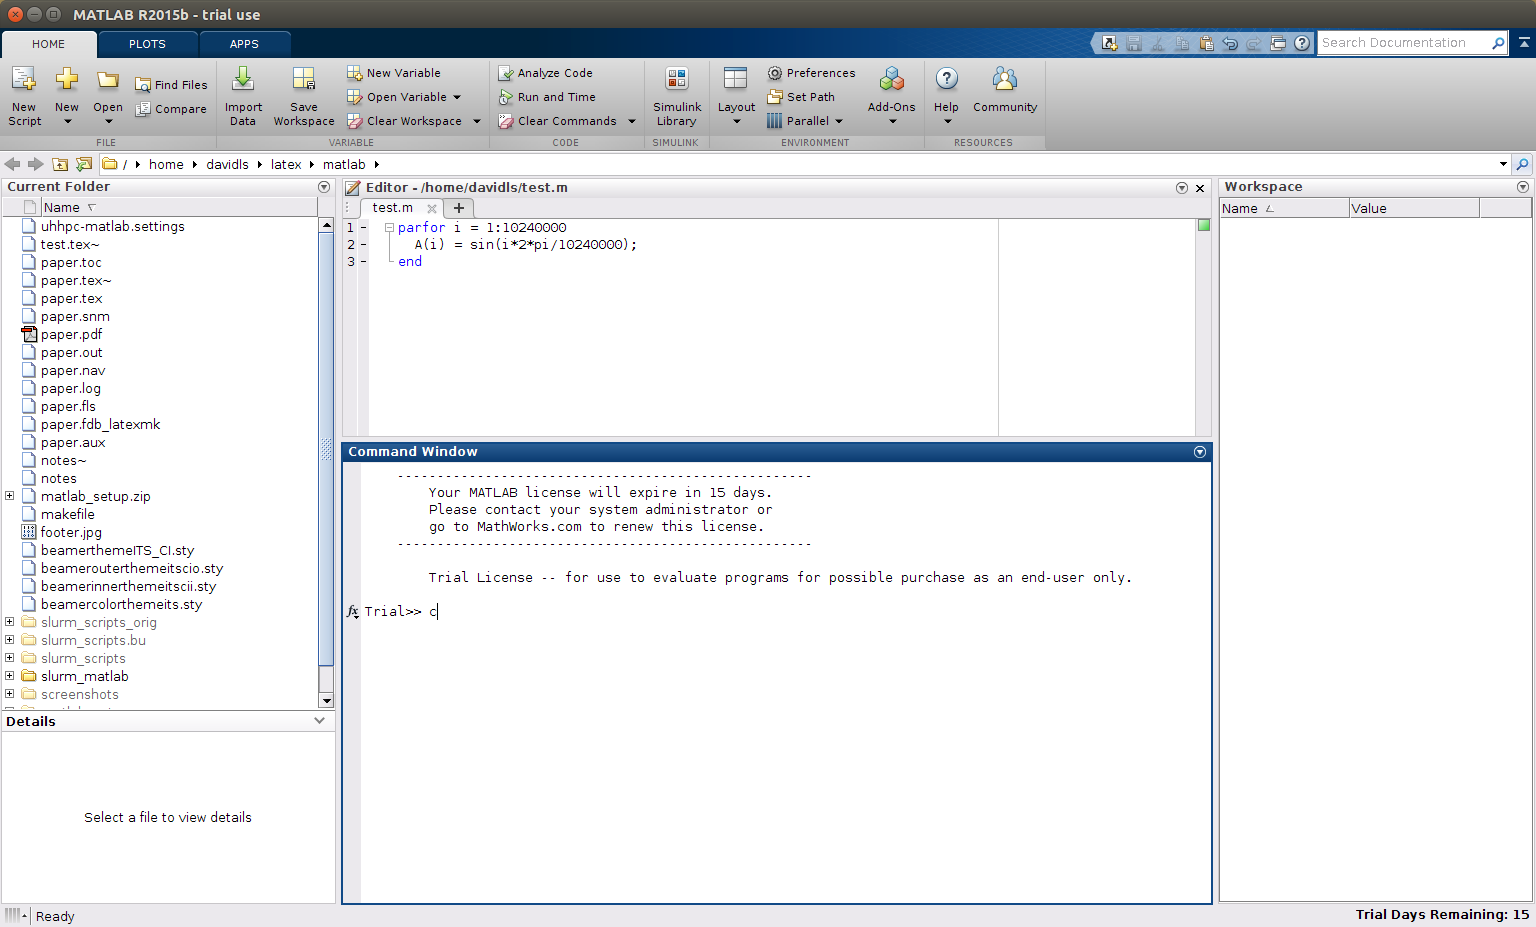
\includegraphics[width=0.8\linewidth]{screenshots/set_path_button}}}
    \only<1>{\put (126,236.5){
\begin{tikzpicture}\draw[red,thick,solid] (0,0) -- (0.6,0) -- (0.6,0.2) -- (0,0.2) -- (0,-0.01);\end{tikzpicture}}}

    \onslide<2-3>{\put (-8,92){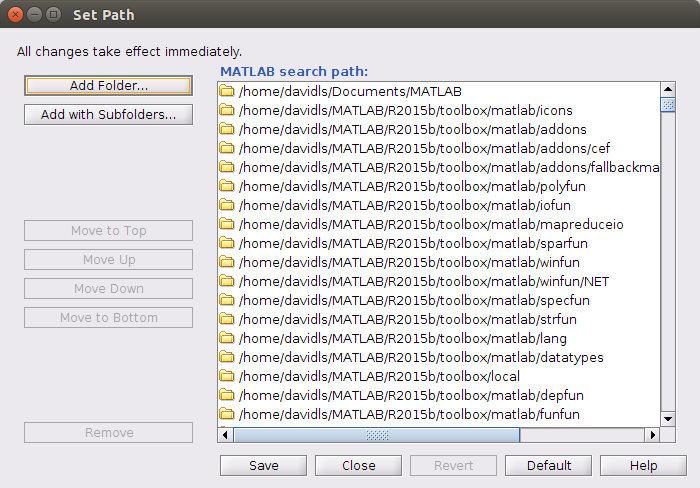
\includegraphics[width=0.4\linewidth]{screenshots/Set_path_window}}}
    \only<2>{\put (-4.25,167.2){
\begin{tikzpicture}\draw[red,thick,solid] (0,0) -- (1.2,0) -- (1.2,0.2) -- (0,0.2) -- (0,-0.01);\end{tikzpicture}}}
    
    \onslide<3>{\put (55,135){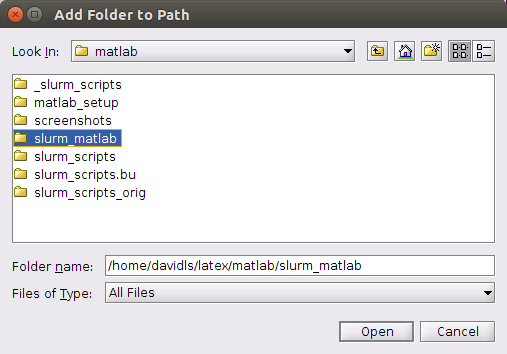
\includegraphics[width=0.35\linewidth]{screenshots/select_path}}}
    \only<3>{\put (78.5,151.7){
\begin{tikzpicture}\draw[red,thick,solid] (0,0) -- (2.2,0) -- (2.2,0.25) -- (0,0.25) -- (0,-0.01);\end{tikzpicture}}}
    \only<3>{\put (133.5,136.5){
\begin{tikzpicture}\draw[red,thick,solid] (0,0) -- (0.7,0) -- (0.7,0.22) -- (0,0.22) -- (0,-0.01);\end{tikzpicture}}}
    
    \onslide<4->{\put (-19,92){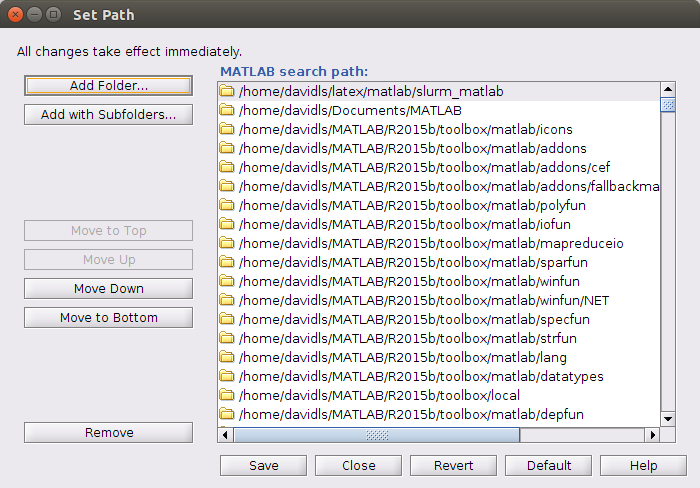
\includegraphics[width=0.4\linewidth]{screenshots/Save_addition}}}
    \only<4>{\put (22.3,166.5){
\begin{tikzpicture}\draw[red,thick,solid] (0,0) -- (3.2,0) -- (3.2,0.3) -- (0,0.3) -- (0,-0.01);\end{tikzpicture}}}
    \only<4>{\put (22.3,92.8){
\begin{tikzpicture}\draw[red,thick,solid] (0,0) -- (1.33,0) -- (1.33,0.2) -- (0,0.2) -- (0,-0.01);\end{tikzpicture}}}
    
    \put(-10,82){
      \begin{minipage}[t]{0.95\linewidth}
        {
          \only<1>{\normalsize{Click the ``\textbf{Set Path}'' button under the ``\textbf{Home}'' tab in\\the MATLAB UI}}
          \only<2>{\normalsize{In the Set Path dialogue, click ``\textbf{Add Folder \ldots}'' }}
          \only<3>{\normalsize{In the Add Folder to Path dialogue, navigate to the directory\\the \textbf{slurm\_matlab} folder resides in and select and \textbf{Open} it}}
          \only<4>{\normalsize{The newly added path should appear in the ``\textbf{MATLAB search path:}'' list.  Once it added, go ahead and click ``\textbf{Save}'', then ``\textbf{Close}''}}
        }
      \end{minipage}
    }
  \end{picture}
\end{frame}


\subsection{Importing \CNAME~MATLAB profile}
\begin{frame}
  \frametitle{Cluster Profile Setup}
  \begin{picture}(320,250)
    \onslide<1,3->{\put(-8,92){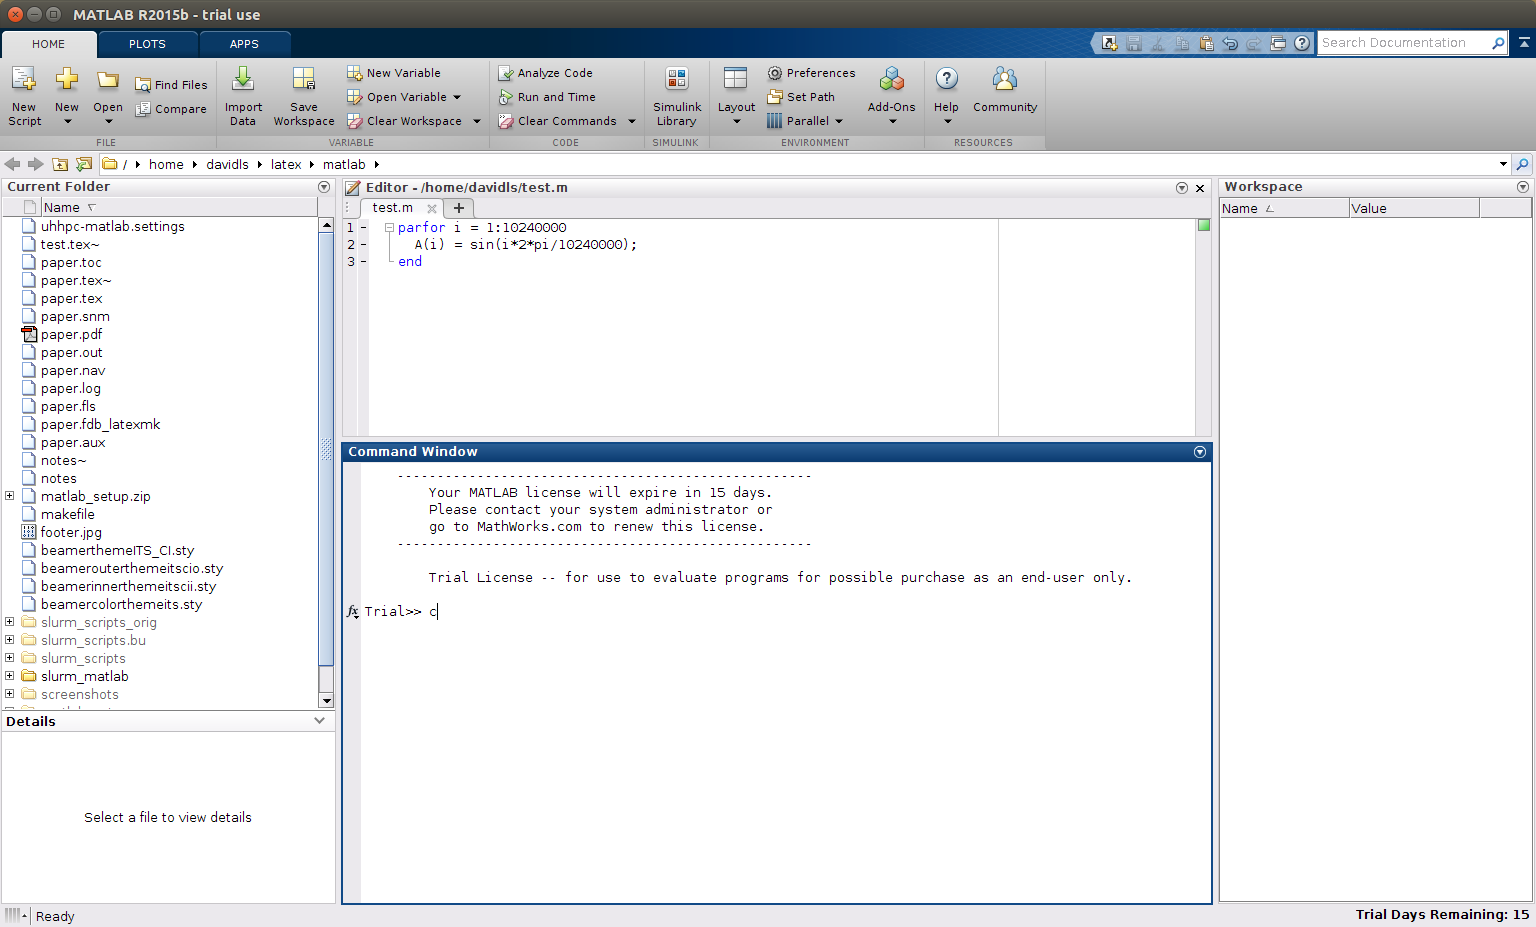
\includegraphics[width=0.8\linewidth]{screenshots/set_path_button}}}
    \only<1>{\put (126,232){
\begin{tikzpicture}\draw[red,thick,solid] (0,0) -- (0.6,0) -- (0.6,0.2) -- (0,0.2) -- (0,-0.01);\end{tikzpicture}}}
    \onslide<2>{\put(-8,92){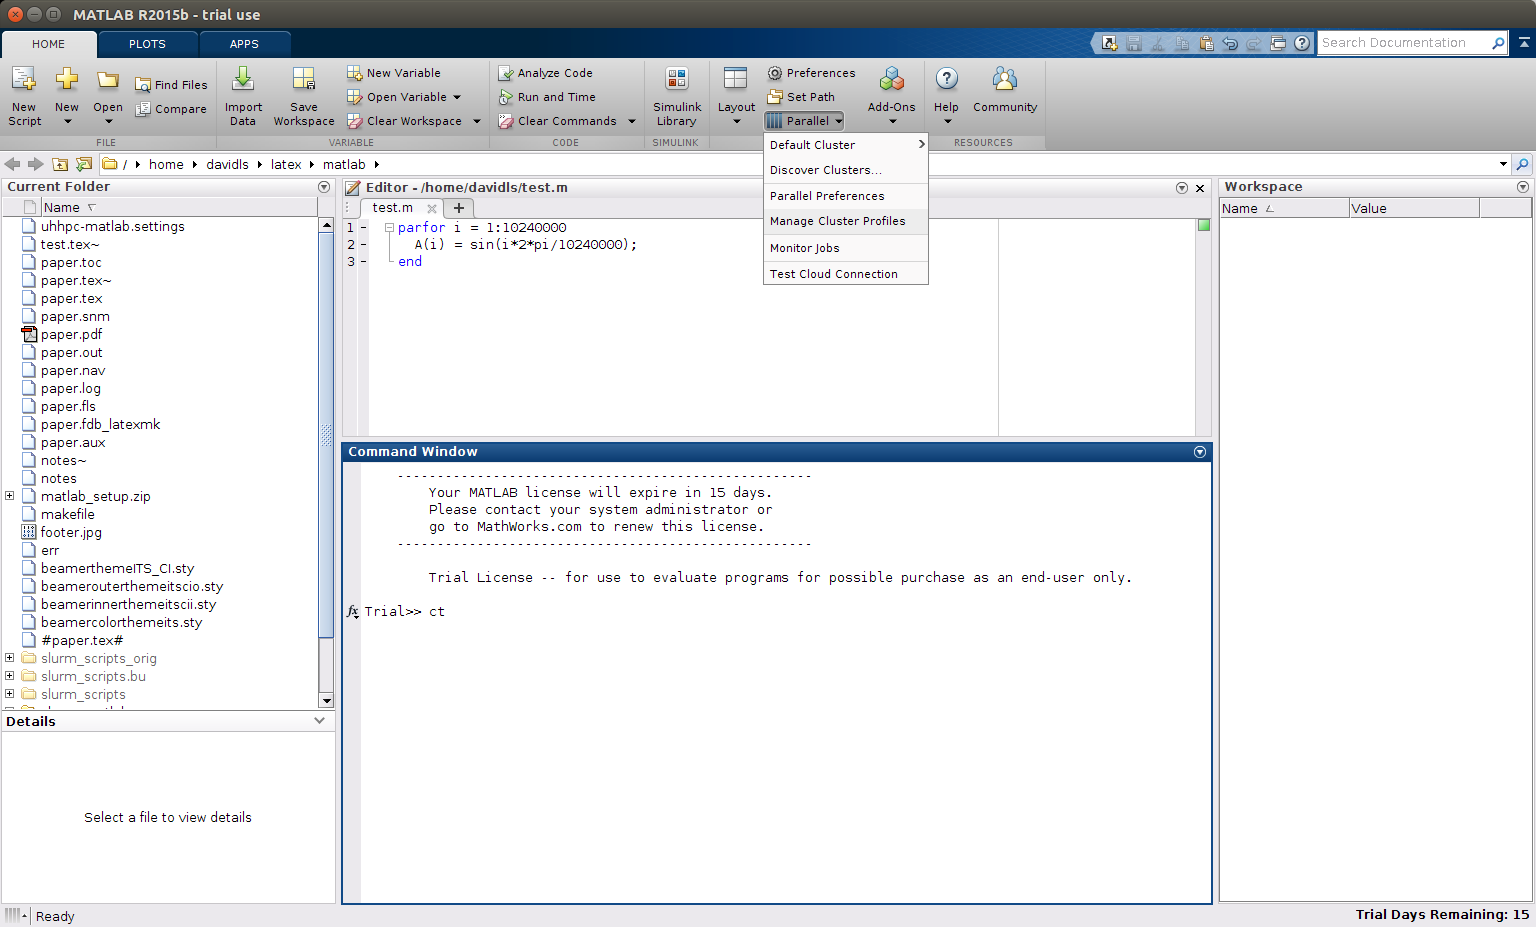
\includegraphics[width=0.8\linewidth]{screenshots/manage_profile}}}
    \only<2>{\put (128,214){
\begin{tikzpicture}\draw[red,thick,solid] (0,0) -- (1,0) -- (1,0.2) -- (0,0.2) -- (0,-0.01);\end{tikzpicture}}}
    \onslide<3-4>{\put(-8,92){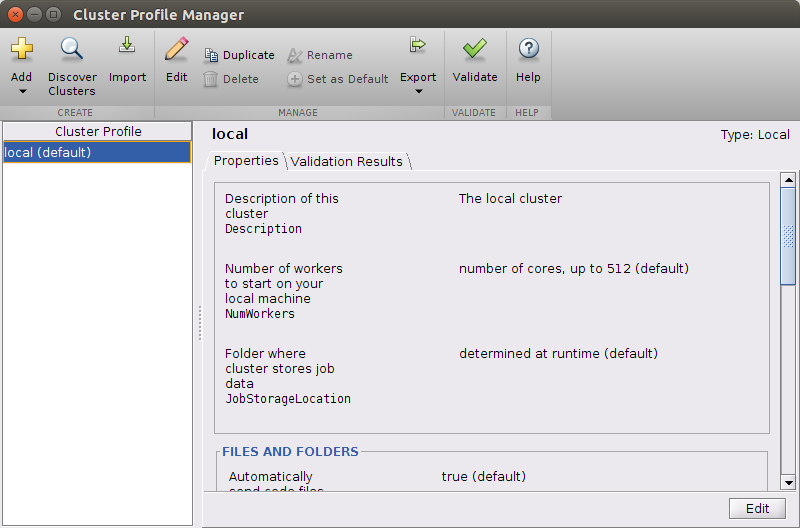
\includegraphics[width=0.4\linewidth]{screenshots/CPM_1}}}
    \only<3>{\put (9.2,163.5){
\begin{tikzpicture}\draw[red,thick,solid] (0,0) -- (0.3,0) -- (0.3,0.46) -- (0,0.46) -- (0,-0.01);\end{tikzpicture}}}
    \onslide<4>{\put(55,135){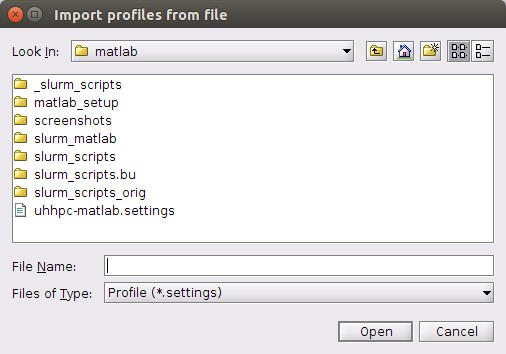
\includegraphics[width=0.35\linewidth]{screenshots/CPM_2}}}
    \only<4>{\put (57,165){
\begin{tikzpicture}\draw[red,thick,solid] (0,0) -- (1.5,0) -- (1.5,0.2) -- (0,0.2) -- (0,-0.01);\end{tikzpicture}}}
    \only<4>{\put (133.5,136.5){
\begin{tikzpicture}\draw[red,thick,solid] (0,0) -- (0.7,0) -- (0.7,0.22) -- (0,0.22) -- (0,-0.01);\end{tikzpicture}}}
    \onslide<5,9>{\put(-8,92){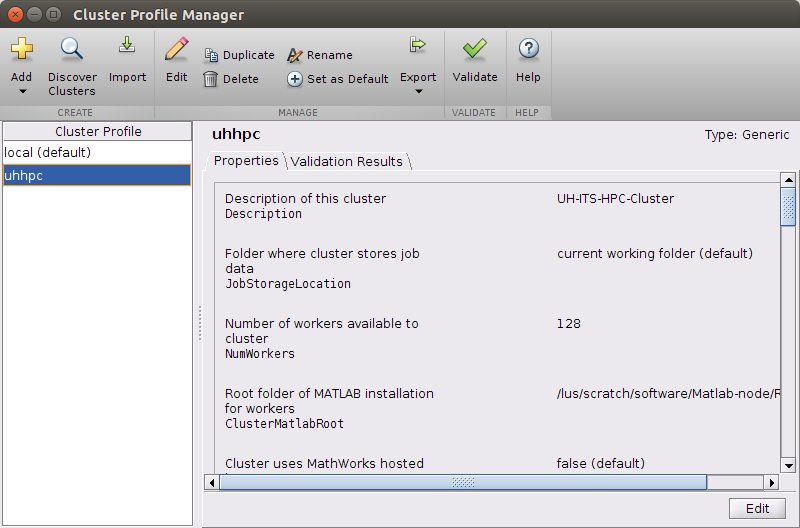
\includegraphics[width=0.4\linewidth]{screenshots/CPM_3}}}
    \only<5>{\put (-8.2,149.65){
\begin{tikzpicture}\draw[red,thick,solid] (0,0) -- (1.15,0) -- (1.15,0.15) -- (0,0.15) -- (0,-0.01);\end{tikzpicture}}}
    \only<5>{\put (115.6,92.4){
\begin{tikzpicture}\draw[red,thick,solid] (0,0) -- (0.4,0) -- (0.4,0.16) -- (0,0.16) -- (0,-0.01);\end{tikzpicture}}}
    \onslide<6>{\put(-8,92){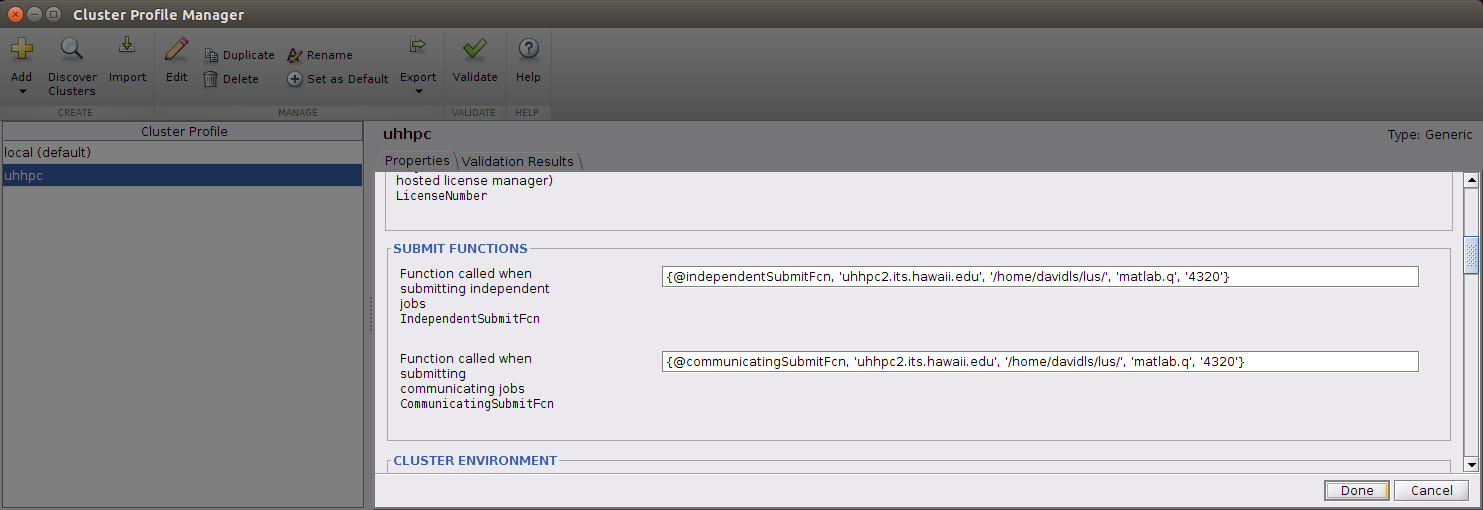
\includegraphics[width=0.8\linewidth]{screenshots/CPM_4}}}
    \onslide<7>{\put(-8,92){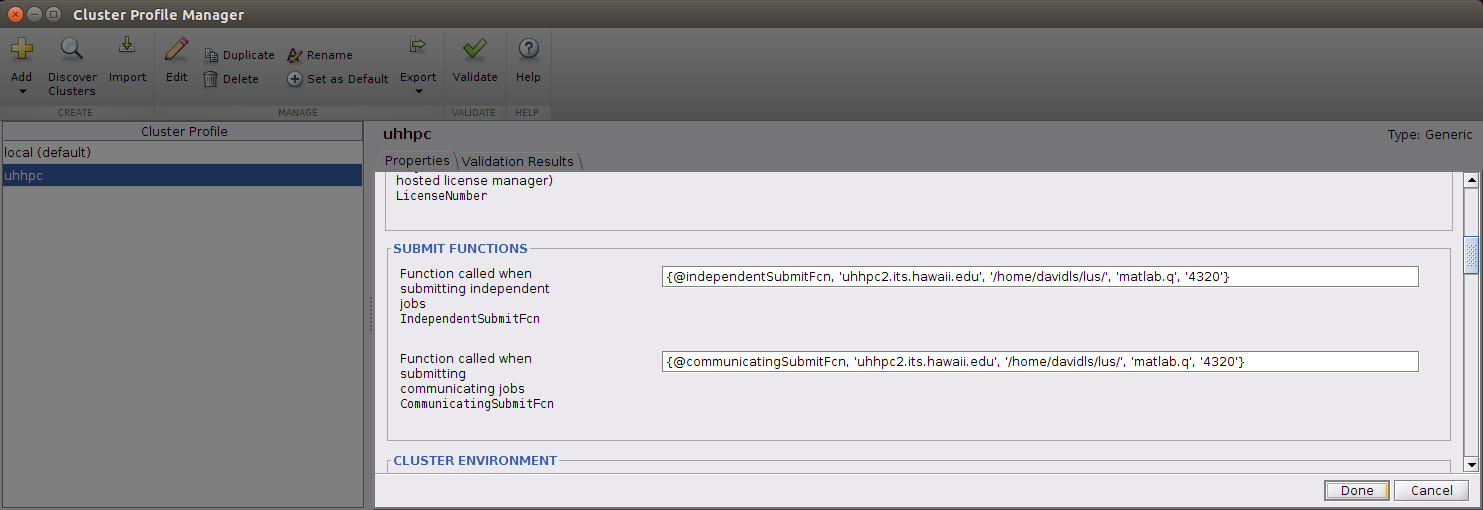
\includegraphics[width=0.8\linewidth]{screenshots/CPM_4}}}
    \onslide<8>{\put(-8,92){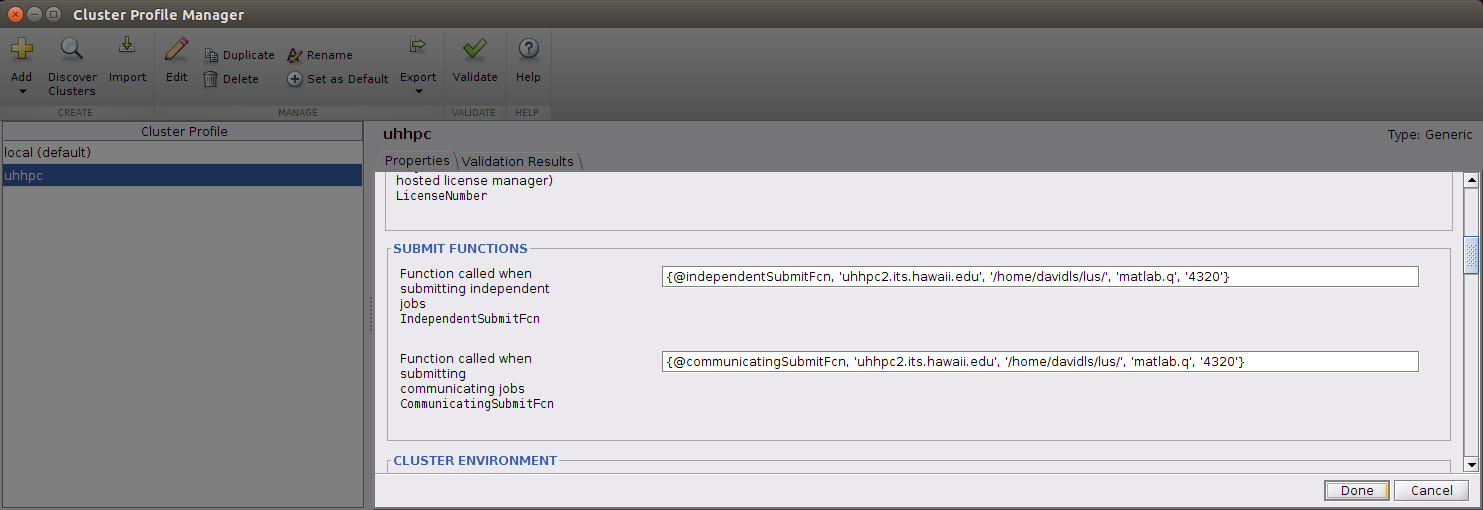
\includegraphics[width=0.8\linewidth]{screenshots/CPM_4}}}
    \put(-20,82){
      \begin{minipage}[t]{0.95\linewidth}
        {
          \only<1>{\normalsize{Click the ``\textbf{Parallel}'' button to bring up the Parallel drop down menu}}
          \only<2>{\normalsize{Select \textbf{Manage Cluster Profiles} in the Parallel drop down menu }}
          \only<3>{\normalsize{In the \textbf{Cluster Profile Manager} dialogue box, click on\\the ``\textbf{Import}'' icon}}
          \only<4>{\normalsize{Navigate to and \textbf{Open} the uhhpc-matlab.settings file\\that was downloaded}}
          \only<5>{\normalsize{Select the \textbf{uhhpc} cluster profile, and press the ``\textbf{Edit}'' button.\\For ease of editing, you may want to increase the window size}}
          \only<6>{\footnotesize{Each of the functions in the \textbf{SUBMIT FUNCTIONS} section, have the follow format:}\\
            \textbf{\tiny{\{$<$func$>$,`$<$server addr$>$', `$<$remote storage dir$>$', `$<$partition$>$', `$<$timelimit$>$', [$<$mem usage in MB$>$] \} } }
          }
          \only<7>{\normalsize{\textbf{\tiny{\{`$<$func$>$',`$<$server addr$>$', `$<$remote storage dir$>$', `$<$partition$>$', `$<$timelimit$>$', [$<$mem usage in MB$>$] \}}}\\Replace the remote storage dir with the path that matches your users lus folder location i.e., /home/$<$username$>$/lus/}}
          \only<8>{\normalsize{\textbf{\tiny{\{`$<$func$>$',`$<$server addr$>$', `$<$remote storage dir$>$', `$<$partition$>$', `$<$timelimit$>$', [$<$mem usage in MB$>$] \}}}\\Adjust the slurm partition and slurm timelimit to fit the partition you wish to run on, and finally click \textbf{done}}}
					\only<9>{\normalsize{The profile should now be configured for your user on \CNAME }}
        }
      \end{minipage}
    }
  \end{picture}
\end{frame}

\begin{frame}
  \frametitle{Cluster Profile}
	\begin{itemize}
	\item To simplify the use of MATLAB on the cluster, we suggest setting the UHHPC cluster profile as the default profile
	\begin{itemize}
		\item Many of the parallel toolbox commands will use the default cluster when an alternate cluster object is not provided
	\end{itemize}
	\item If the UHHPC cluster profile is not set as the default, the cluster profile name, \textbf{`uhhpc'}, must be provided when creating the cluster object
	\item If you plan to change partitions or run in multiple partitions on \CNAME, you will need to modify the existing profile, or create duplicate profiles with the required changes to the remote storage location, partition and timelimit
	\end{itemize}
	
\end{frame}

%------------------------------------------------
\section{Basic Commands \& Testing}

\subsection{Commands}
\begin{frame}
\frametitle{Commands}
\begin{itemize}
\item \href{http://www.mathworks.com/help/distcomp/pctconfig.html}{pctconfig} -- Configure settings for Parallel Computing Toolbox client session
  \begin{itemize}
  \item[-] Is not persistent
  \item[-] Must be set before any interaction with the parallel toolbox occurs
  \item[-] Used to set the correct 'hostname' in MATLAB\\e.g.,~$>$~pctconfig(`hostname', `192.168.0.1')
		\begin{itemize}
		\item[-] A valid `hostname' is required for validation to pass as well as for many of the parallel functions to work
		\end{itemize}
  \end{itemize}
\item \href{http://www.mathworks.com/help/distcomp/parcluster.html}{parcluster} -- Creates a cluster object which can be passed to functions used to create parallel tasks
\item \href{http://www.mathworks.com/help/distcomp/gcp.html}{gcp} -- Get current parallel pool
\item \href{http://www.mathworks.com/help/distcomp/addattachedfiles.html}{addAttachedFiles} -- Attach files or folders to parallel pool
\end{itemize}
\end{frame}


\begin{frame}
	\frametitle{Commands}
	\begin{itemize}
	\item \href{http://www.mathworks.com/help/distcomp/batch.html}{batch} -- Run MATLAB script or function on worker
		\begin{itemize}
		\item Non-interactive.  MATLAB can be closed
		\end{itemize}
	\item \href{http://www.mathworks.com/help/distcomp/parpool.html}{parpool} -- Create parallel pool on cluster
	\item \href{http://www.mathworks.com/help/distcomp/spmd.html}{spmd} -- Execute code in parallel on workers of parallel pool
	\end{itemize}
	For more information and other commands, visit the\\\href{http://www.mathworks.com/help/distcomp}{\textbf{Distributed toolbox help manual}} on the MathWorks website
\end{frame}


\subsection{Validation}
\begin{frame}
\frametitle{Simple Tests}
\begin{itemize}
\item Simplest test is to use ``\emph{validate}'' in the \textbf{Cluster Profile Manager}
\item Before testhing, make sure to reduce the value for ``Number of workers available to cluster''~(NumWorkers) value to something lower than \TOTWRKS{}
  \begin{itemize}
  \item[-] Typically we test with 2 -- 10 workers
  \end{itemize}
\item NumWorkers must be lowered since validate uses this as the number of workers to request
\item You also must make sure the hostname in MATLAB is set correctly (using~pctconf), or the parpool test may fail
\item Remember to reset the NumWorkers value back to \TOTWRKS{} or you may get errors saying not enough workers when requesting more than the current NumWorkers value
\end{itemize}\end{frame}

\section{Demo}
\begin{frame}
\frametitle{Demo}
\huge{\centerline{Live Demo \ldots}}
\end{frame}

\section{Resources}
\begin{frame}
\frametitle{Resources}
\begin{itemize}
\item Newest revision of these slides -- \url{http://go.hawaii.edu/H5}
\item \href{https://rc.fas.harvard.edu/resources/documentation/software/parallel-matlab-pct-dcs/}{Parallel MATLAB (PCT and DCS)} @ Harvard
\begin{itemize}
	\item Not all sections pertain to our cluster, but some sections provide some information on running jobs with the parallel toolbox
	\item The \href{https://rc.fas.harvard.edu/resources/documentation/software/parallel-matlab-pct-dcs/\#Submitting_DCS_jobs_from_within_MATLAB}{``Submitting DCS jobs from within MATLAB''} section covers using the batch command to submit parallel jobs to a cluster
\end{itemize}
\end{itemize}
\end{frame}

\begin{frame}
\huge{\centerline{Questions?}}
\end{frame}

%----------------------------------------------------------------------------------------

\end{document}
